\documentclass{article}
\usepackage[catalan]{babel}
\usepackage[a4paper, total={6.5in, 9.5in}]{geometry}
\usepackage{multirow}
\usepackage{graphicx}
\usepackage[backend=biber, style=numeric,sorting=nty]{biblatex}

\begin{document}

\nocite{*}

\title{\textbf{Implementació d'un Sistema RISC-V en \textit{FPGA} amb suport per \textit{Linux}} \\
Informe de seguiment I}
\author{Oscar Lostes Cazorla}
\date{Novembre 2021}

\clearpage\maketitle
\thispagestyle{empty}

\newpage

\section{Comparativa d'objectius respecte l'informe inicial}

A l'anterior informe es van exposar les següents decisions:
\begin{itemize}
\item Ús d'Ubuntu com a distribució \textit{Linux}.
\item Ús del \textit{softcore} NOEL-V de Gaisler com a processador.
\end{itemize}

La part de \textit{Linux} encara no ha estat explorada en profunditat, i per tant es manté l'objectiu com a pendent.

Per altra banda, s'han centrat els esforços en la part \textit{hardware} del projecte: el \textit{softcore}. A l'informe inicial es va establir que NOEL-V semblava la millor opció, però després de realitzar una investigació i experimentació més exhaustiva s'ha acabat desistint d'emprar aquesta tecnologia pels següents motius:

\begin{itemize}
\item La GRLIB (llibreria de Gaisler on es troba el NOEL-V) presenta suport per a plaques Altera, però només ofereix projectes pregenerats per al LEON3 (un altre processador de la companyia).
Això implica que s'ha de generar tot de zero, i si bé no és inherentment un problema, en conjunt amb la resta de motius sí que ho és.
\item NOEL-V, i el \textit{SoC} que s'implementa al seu voltant és massa gran (en recursos de la \textit{FPGA}) per a qualsevol de les plaques de què es disposen actualment per al projecte.
\item La GRLIB proporciona una interfície de configuració (tant gràfica com textual) bastant limitada. Alguns dels components que es voldrien configurar per a reduir l'ús de recursos es troben \textit{hardcoded} al disseny i no es poden canviar fàcilment.
\item \textit{Quartus} treballa, principalment, amb el bus de comunicacions AXI, mentre que el NOEL-V empra el bus AMBA.
\end{itemize}

A més, el codi VHDL de la llibreria no permet connectar de forma fàcil dispositius externs a la \textit{FPGA} (com poden ser la RAM o la SD, en aquest cas). Per superar aquest problema, es va decidir generar un component per al dissenyador de plataformes de Quartus (\textit{Qsys}). Però a l'hora de dur a terme aquesta tasca es presenta un problema de dependències amb un cert component de la llibreria, que no s'ha pogut trobar enlloc (ni als arxius, ni a la documentació ni a Internet) i fa impossible la generació d'aquest component.\\

Per tots aquests motius, es desestima NOEL-V com a \textit{softcore} candidat, s'atura la seva investigació i es decideix moure el projecte cap a altres tecnologies.

\section{Estat actual: \textit{Chipyard}}

Ja que NOEL-V ha deixat de ser una opció viable, s'ha començat a explorar la següent alternativa proposada: \textit{Chipyard}.\\

\textit{Chipyard} és un \textit{framework} de simulació i síntesi de sistemes RISC-V, que aglutina diverses eines i llibreries en un sol paquet. Tot i oferir-se en altres formes d'us, el \textit{framework} es distribueix en format \textit{Docker} amb les eines precompilades i preparades. Per la facilitat d'us que proporciona aquest entorn de contenidor, s'opta per aquesta via.\\

Tal i com es va comentar a l'informe anterior, aquesta eina permet la generació de sistemes basats (entre d'altres) en els \textit{cores} Rocket, BOOM i CVA6/Ariane. En una consulta preliminar a la documentació del projecte, s'ha pogut determinar que el suport per a CVA6 és un dels més limitats, i per aquest motiu, es descarta pel ara. D'entre les altres dues opcions, s'ha començat a experimentar amb sistemes basats en Rocket, ja que BOOM (pel fet de ser un nucli fora d'ordre) pot ser potencialment més gran (i ja s'ha establert que la quantitat de recursos és un factor crític).\\

El generador Rocket Chip (es a dir, el \textit{SoC} basat en Rocket Core) està inclòs a \textit{Chipyard}. Aquest generador està basat en Chisel: un llenguatge de descripció de hardware implementat en Scala. D'aquesta forma, no obtenim un codi VHDL/Verilog directament, sinó que aquest codi es genera en base a les nostres especificacions. Si bé, idealment, no s'haurà de programar res en Chisel, és bo saber que aquesta és la tecnologia subjacent, ja que amb petits canvis d'aquest codi es podran realitzar canvis en la configuració del \textit{SoC}.\\

Actualment s'estan realitzant proves amb el sistema per defecte que deixa generar \textit{Chipyard}. A la figura \ref{fig:rocketchip}, es pot veure una representació en alt nivell del sistema que s'obté:\\

\begin{figure}[h]
\centering
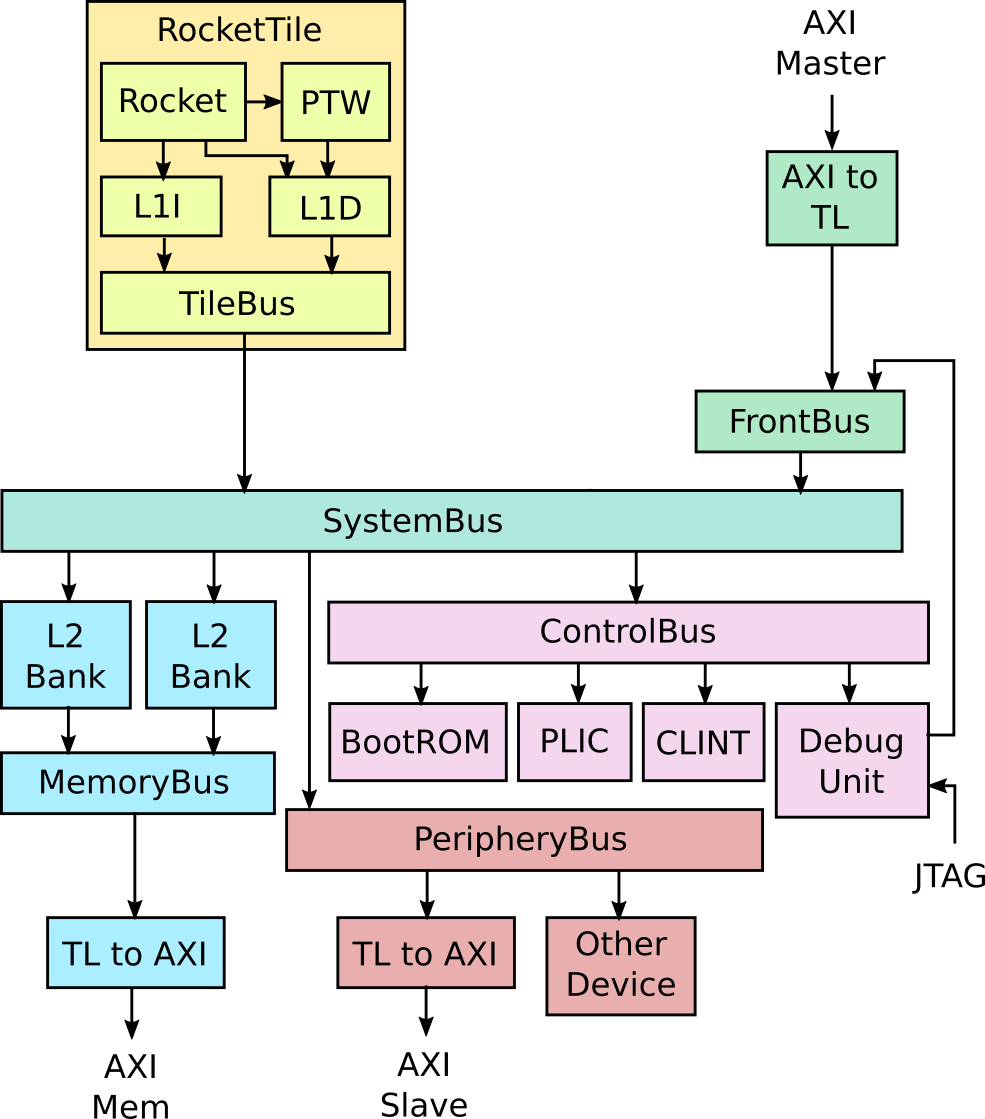
\includegraphics[width=8cm]{rocketchip-diagram.png}
\caption{Rocket Chip per defecte}
\label{fig:rocketchip}
\end{figure}

Podem veure que aquest sistema proporciona tots els dispositius bàsics que es puguin necessitar, i també ens proporciona un factor clau: interconnexió amb el bus AXI, tan per a memòria principal com per a perifèrics. 
Aixo significa, que de cara a muntar un sistema sencer amb RAM, memòria secundària (SD), sortida de vídeo i teclat/ratolí, es pot generar un component \textit{Qsys} amb aquest \textit{SoC} i integrar-lo fàcilment amb tots aquests dispositius.\\

Actualment s'han aconseguit les següents fites envers aquesta part del projecte:
\begin{itemize}
    \item Insta\lgem ació del \textit{Docker} de \textit{Chipyard}.
    \item Generació del codi Verilog del Rocket Chip per defecte.
    \item Importació, anàlisi i síntesi dins d'un projecte Quartus.
\end{itemize}

\section{Següents passos}

En el punt actual del projecte, les següents fites a aconseguir a curt termini són:
\begin{itemize}
    \item Determinar si el \textit{SoC} per defecte compleix els requisits de recursos com per a cabre a les nostres plaques, i fer els canvis de configuració necessaris si s'escau.
    \item Creació del component \textit{Qsys} a partir del \textit{SoC}.
    \item Integració del \textit{SoC} amb la resta de dispositius del sistema.
    \item Programació efectiva de la \textit{FPGA}, on el sistema fos capaç d'executar algun software (encara que sigui \textit{baremetal} directament des de la BootROM)
\end{itemize}

Si s'aconsegueixen aquestes fites, es podrà passar de forma efectiva a la següent fase del projecte, on s'intenti executar \textit{Ubuntu} sobre aquest sistema.

% \newpage

% \printbibliography[title={Bibliografia web}]

\end{document}